\documentclass[11pt,a4paper]{article}

\usepackage[margin=1in]{geometry}
\usepackage{amsmath,amssymb}
\usepackage{graphicx}
\usepackage{booktabs}
\usepackage{xcolor}
\usepackage[colorlinks=true,linkcolor=blue!50!black,citecolor=blue!50!black,
            urlcolor=blue!50!black]{hyperref}

\newcommand{\lon}{\mathrm{lon}}
\newcommand{\dt}{\delta_t}
\newcommand{\de}{\delta_e}

\title{\textbf{Longitudinal Dynamics and Control of a Fixed-Wing UAV}\\[2mm]
\large Trim, Linearisation, Modal Analysis and Autopilot Design}
\author{Sashank\\[1mm]\small AE695 --- State Space Analysis and Design\\
\small Indian Institute of Technology Bombay}
\date{\today}

\begin{document}
\maketitle

\begin{abstract}
\noindent
This report implements the complete longitudinal design chain of Beard and
McLain~\cite{beard}, chapters 3 to 6, for a fixed-wing unmanned aircraft: the
nonlinear five-state plant, trim, linearisation about trim, transfer function
models, the reduced-order short-period and phugoid approximations, and a
successive-loop-closure autopilot. Everything is implemented in base MATLAB with
no toolbox dependencies.

Two airframes are carried in parallel: the Aerosonde of the reference text, and a
canard configuration taken from an existing six-degree-of-freedom Simulink model.
Trim is solved to a residual of $\sim\!2\times10^{-15}$ for both. The linearised
model reproduces the published reference matrices to $3.8\times10^{-5}$
($A_\lon$) and $1.4\times10^{-10}$ ($B_\lon$), and the analytic transfer function
coefficients $a_{\theta_1}$ through $a_{\theta_3}$ match to seven significant
figures.

Two defects in the reference material are documented. Its companion code contains
no implemented physics, and its published trim point is not a force equilibrium:
evaluating the dynamics there gives $\dot u = -0.85\,\mathrm{m/s^2}$, because the
propeller model delivers about $0.95\,\mathrm{N}$ against $10.3\,\mathrm{N}$ of
drag. The verification strategy was restructured around both findings.
\end{abstract}

\tableofcontents
\clearpage

%======================================================================
\section{Scope and approach}

The full rigid-body aircraft has twelve states. Chapter 5 of~\cite{beard}
decouples these into a lateral set $(v,p,r,\phi,\psi)$ and a longitudinal set
$(u,w,q,\theta,h)$, leaving north and east position as pure navigation states
that appear in neither. This report takes the longitudinal set only.

The decoupling is obtained by forcing every lateral state to zero,
\begin{equation}
  v = p = r = \phi = \psi = \beta = 0,
  \label{eq:decouple}
\end{equation}
together with zero wind. Under~\eqref{eq:decouple} the Euler kinematics collapse
from $\dot\theta = q\cos\phi - r\sin\phi$ to simply $\dot\theta = q$.

A consequence worth stating at the outset: the only attitude variable remaining is
$\theta$, which is an Euler angle with no singularity anywhere in the
longitudinal flight envelope. The quaternion formulation that the reference text's
companion code uses for its thirteen-state propagation, together with its
quaternion-to-Euler conversion layer, is therefore unnecessary here and has been
omitted. This removes the most error-prone part of the reference implementation
without any loss of generality in the longitudinal plane.

\subsection{State and input}

\begin{equation}
  x_\lon = \begin{bmatrix} u & w & q & \theta & h \end{bmatrix}^{\!\top},
  \qquad
  u_\lon = \begin{bmatrix} \de & \dt \end{bmatrix}^{\!\top},
  \label{eq:state}
\end{equation}
with body-axis velocities in $\mathrm{m/s}$, pitch rate in $\mathrm{rad/s}$,
pitch angle in $\mathrm{rad}$, altitude in $\mathrm{m}$, elevator in
$\mathrm{rad}$ and throttle on $[0,1]$.

Altitude is carried as a state rather than down-position $p_d$. This is a
deliberate choice: the reference implementation integrates $p_d$ and must then
negate a row and a column of its Jacobian to report $A_\lon$ in the ordering
of~\eqref{eq:state}. Integrating $h$ directly makes that post-processing step
vanish, and the Jacobian emerges in the book's ordering and sign convention with
no manipulation at all.

%======================================================================
\section{Nonlinear longitudinal model (chapters 3 and 4)}

\subsection{Equations of motion}

Reducing book equations (5.3), (5.4), (5.6) and (5.11)
under~\eqref{eq:decouple} gives
\begin{align}
  \dot u      &= -qw + f_x/m, \label{eq:udot}\\
  \dot w      &= \phantom{-}qu + f_z/m, \label{eq:wdot}\\
  \dot q      &= M_y/J_y, \label{eq:qdot}\\
  \dot\theta  &= q, \label{eq:thetadot}\\
  \dot h      &= u\sin\theta - w\cos\theta. \label{eq:hdot}
\end{align}
The pitch equation~\eqref{eq:qdot} is a genuine simplification rather than an
approximation: the general form carries $\Gamma_5 pr + \Gamma_6(p^2-r^2)$, both of
which vanish identically when $p=r=0$.

Air data follows from the velocity components,
\begin{equation}
  V_a = \sqrt{u^2+w^2}, \qquad \alpha = \operatorname{atan2}(w,u).
  \label{eq:airdata}
\end{equation}
The two-argument arctangent is used in place of $\arctan(w/u)$. The two agree for
$u>0$ but only the former stays finite at $u=0$.

\subsection{Aerodynamic forces and moments}

With $\bar q = \tfrac12\rho V_a^2$ and the non-dimensionalising length
$\hat c = c/(2V_a)$,
\begin{align}
  C_L &= C_{L}(\alpha) + C_{L_q}\hat c\, q + C_{L_{\de}}\de, \label{eq:CL}\\
  C_D &= C_{D}(\alpha) + C_{D_q}\hat c\, q + C_{D_{\de}}\de, \label{eq:CD}\\
  C_m &= C_{m_0} + C_{m_\alpha}\alpha + C_{m_q}\hat c\, q + C_{m_{\de}}\de.
  \label{eq:Cm}
\end{align}

Two remarks on~\eqref{eq:Cm}. First, the correct non-dimensionalising length for
the pitch-damping term is the \emph{chord}. Using the span instead is an error
present in some existing fixed-wing Simulink models, and it over-weights pitch
damping by the ratio $b/c$, roughly a factor of five for the canard geometry
considered here. Second, $C_{m_0}$ in~\eqref{eq:Cm} is a zero-incidence
derivative, not the constant term of a polynomial fit; the two meanings collide
in some parameter files and a model can compile with the wrong one and still be
silently wrong.

Lift and drag act in the wind frame and are rotated into body axes, after which
gravity and thrust are added:
\begin{align}
  f_x &= -mg\sin\theta + \bigl(-D\cos\alpha + L\sin\alpha\bigr) + T,
  \label{eq:fx}\\
  f_z &= \phantom{-}mg\cos\theta + \bigl(-D\sin\alpha - L\cos\alpha\bigr).
  \label{eq:fz}
\end{align}
Thrust appears only in~\eqref{eq:fx}. That it is absent from~\eqref{eq:fz} is not
incidental; it is the structural fact that makes the trim computation of
Section~\ref{sec:trim} triangular.

\subsection{Lift model}

For the Aerosonde, lift blends a linear model into a flat-plate model past stall
through the sigmoid of book equations (4.9) and (4.10),
\begin{equation}
  C_L(\alpha) = \bigl(1-\sigma(\alpha)\bigr)
                \bigl(C_{L_0} + C_{L_\alpha}\alpha\bigr)
              + \sigma(\alpha)\,
                2\operatorname{sign}(\alpha)\sin^2\!\alpha\cos\alpha ,
  \label{eq:blend}
\end{equation}
with $\sigma$ the blending function parameterised by $M$ and $\alpha_0$.

For the canard, $\alpha_0$, $M$ and $\epsilon$ were never identified, so the lift
curve is kept linear and the blend is disabled by a flag. No attempt was made to
invent stall parameters. In particular, ``no stall'' must not be encoded as
$\alpha_0\to\infty$, because the sigmoid then evaluates to \texttt{NaN}.

\subsection{Drag model}

Drag is implemented as a polynomial in $\alpha$ evaluated by Horner's method. This
single code path covers both airframes, because the book's linear-in-$\alpha$ drag
is simply a degenerate quadratic:
\begin{equation}
  C_D(\alpha) = \begin{cases}
    0.132\,\alpha + 0.0424 & \text{Aerosonde},\\
    2.8252\,\alpha^2 - 0.0137\,\alpha + 0.0461 & \text{canard}.
  \end{cases}
  \label{eq:dragpoly}
\end{equation}
It is worth recording that the Aerosonde drag is the linear form
and \emph{not} the induced-drag polar $C_{D_p} + C_L^2/(\pi e \mathrm{AR})$. This
was established numerically rather than assumed: only the linear form reproduces
the published $a_{V_1}$, as shown in Section~\ref{sec:verif}. Consequently
$C_{D_p}$, the aspect ratio and the Oswald efficiency are unused.

\subsection{Propulsion}

Two models are implemented, selected per airframe. The Aerosonde uses the
propeller and motor model of the text's addendum: the propeller torque is matched
to the motor torque, which gives a quadratic in propeller speed $\Omega$,
\begin{equation}
  \underbrace{\frac{\rho D^5 C_{Q_0}}{4\pi^2}}_{a}\Omega^2
  + \underbrace{\left(\frac{\rho D^4 C_{Q_1} V_a}{2\pi}
    + \frac{K_Q^2}{R}\right)}_{b}\Omega
  + \underbrace{\rho D^3 C_{Q_2} V_a^2
    - \frac{K_Q V_{\mathrm{in}}}{R} + K_Q i_0}_{c} = 0 ,
  \label{eq:propquad}
\end{equation}
after which thrust follows from the thrust coefficient at the resulting advance
ratio. Equation~\eqref{eq:propquad} is solved as
$\Omega = -2c/\bigl(b+\sqrt{b^2-4ac}\bigr)$ rather than by the textbook quadratic
formula. The two are algebraically identical, but at cruise $4ac \ll b^2$, and the
textbook form then loses most of its significant figures to cancellation.

The canard uses a velocity-lapsed law,
$T = \max\bigl(0,\;T_{\mathrm{static}}(1 - V_a/V_{\max})\dt\bigr)$.

The legacy simple propeller model of chapter 4 is \emph{not} implemented. It
cannot be what generated the published reference values: it yields
$\partial T/\partial V_a = -6.43\,\mathrm{N/(m/s)}$ where $-2.35$ is required.

%======================================================================
\section{Trim}\label{sec:trim}

\subsection{The problem is triangular}

Appendix F.2 of~\cite{beard} shows that for wings-level longitudinal flight the
trim problem decouples completely. Given a target airspeed $V_a^*$ and flight path
angle $\gamma^*$:

\begin{enumerate}
\item $\alpha$ fixes the kinematics:
  $\theta = \alpha + \gamma$, $q = 0$, $u = V_a\cos\alpha$, $w = V_a\sin\alpha$.
\item $\de$ is then available in \emph{closed form} from $\dot q = 0$
  with $q=0$, using~\eqref{eq:qdot} and~\eqref{eq:Cm}:
  \begin{equation}
    \de^* = -\frac{C_{m_0} + C_{m_\alpha}\alpha^*}{C_{m_{\de}}} .
    \label{eq:detrim}
  \end{equation}
\item $\alpha$ follows from a \emph{scalar} root-find on $\dot w = 0$. Because
  thrust is absent from~\eqref{eq:fz}, this step is independent of throttle.
\item $\dt$ follows from a scalar root-find on $\dot u = 0$, solved last.
\end{enumerate}

Altitude needs no equation. Once $\theta = \alpha+\gamma$, substituting
into~\eqref{eq:hdot} gives
\begin{equation}
  \dot h = V_a\cos\alpha\sin(\alpha+\gamma) - V_a\sin\alpha\cos(\alpha+\gamma)
         = V_a\sin\gamma
  \label{eq:hdotauto}
\end{equation}
identically, so the commanded climb rate is satisfied automatically. This is used
as a verification condition in Section~\ref{sec:verif}.

\subsection{Why not an optimiser}

The reference implementation solves trim with \texttt{fmincon} on a seventeen-element
decision vector, because it trims all twelve states simultaneously and must
enforce quaternion normalisation as an explicit constraint. For the longitudinal
plane that is a constrained nonlinear program applied to a problem that is
triangular and has an analytic middle step.

Two scalar \texttt{fzero} calls are used instead. The practical consequences are:
no Optimization Toolbox dependency; a residual at machine precision rather than at
a tolerance one has to choose; and an informative failure mode, since the bracket
$\alpha\in[-0.2,0.3]\,\mathrm{rad}$ is physically meaningful and a sign-change
failure genuinely means no trim exists at that airspeed. The last point matters
downstream, because the Jacobian of Section~\ref{sec:lin} is taken about the trim
point and any trim error propagates directly into it.

\subsection{Results}

\begin{table}[htbp]
\centering
\begin{tabular}{lrr}
\toprule
Quantity & Aerosonde & Canard \\
\midrule
$V_a^*$ [m/s] & $25.00$ & $25.00$ \\
$\alpha^*$ [deg] & $2.8476$ & $-0.3817$ \\
$\theta^*$ [deg] & $2.8476$ & $-0.3817$ \\
$u^*$ [m/s] & $24.9691$ & $24.9994$ \\
$w^*$ [m/s] & $1.2420$ & $-0.1666$ \\
$\delta_e^*$ [deg] & $-7.1000$ & $0.6389$ \\
$\delta_t^*$ & $0.7734$ & $0.1533$ \\
$\lVert f(x^*,u^*)\rVert$ & $1.91\times 10^{-15}$ & $2.96\times 10^{-15}$ \\
\bottomrule
\end{tabular}

\caption{Trim at $V_a^*=25\,\mathrm{m/s}$, $\gamma^*=0$. The residual is
$\lVert f(x^*,u^*)\rVert$ over the first four states, i.e.\ how nearly the
computed point is a true equilibrium.}
\label{tab:trim}
\end{table}

Both airframes trim to machine precision. The canard trims at a slightly
\emph{negative} angle of attack, which is correct for it: its zero-incidence lift
coefficient $C_{L_0}=0.3494$ slightly exceeds the $C_L=0.324$ needed to carry
$2.4\,\mathrm{kg}$ at $25\,\mathrm{m/s}$ on $0.19\,\mathrm{m^2}$, so a small
negative incidence is required to shed the excess.

%======================================================================
\section{Linearisation}\label{sec:lin}

\subsection{Method}

The Jacobians are formed by finite differences about the trim point, following
Appendix F.4. Central differences with a per-variable scaled step
$h_i = 10^{-6}\max(1,|x_i|)$ are used by default, giving second-order accuracy.

A forward-difference mode with a fixed step of $0.01$ is also provided, used
only for the reference comparison in Section~\ref{sec:verif}: the published
matrices were generated that way, and reproducing them requires reproducing their
differencing scheme. That step is far too large for accuracy and is deliberately
not the default. Matching a reference's discretisation error is not the same as
being correct, and the two should not be conflated.

\subsection{Results}

For the Aerosonde at $V_a^*=25\,\mathrm{m/s}$, in the ordering
of~\eqref{eq:state}:
\begin{equation}
  A_\lon = \begin{bmatrix}
    -0.2821 & 0.4949 & -1.2123 & -9.7979 & 0 \\
-0.5611 & -4.4978 & 24.3714 & -0.4874 & 0 \\
0.1986 & -3.9930 & -5.2947 & 0 & 0 \\
0 & 0 & 1.0000 & 0 & 0 \\
0.0497 & -0.9988 & 0 & 25.0000 & 0

  \end{bmatrix},
  \qquad
  B_\lon = \begin{bmatrix}
    -0.1392 & 9.4800 \\
-2.5861 & 0 \\
-36.1124 & 0 \\
0 & 0 \\
0 & 0

  \end{bmatrix}.
  \label{eq:Aaero}
\end{equation}

For the canard:
\begin{equation}
  A_\lon = \begin{bmatrix}
    -0.1480 & 0.4194 & 0.1624 & -9.8138 & 0 \\
-0.8219 & -5.5224 & 24.3736 & 0.0654 & 0 \\
-0.0150 & -2.2541 & -3.7468 & 0 & 0 \\
0 & 0 & 1.0000 & 0 & 0 \\
-0.0067 & -1.0000 & 0 & 25.0000 & 0

  \end{bmatrix},
  \qquad
  B_\lon = \begin{bmatrix}
    -1.9051 & 9.2900 \\
-13.0192 & 0 \\
-221.0583 & 0 \\
0 & 0 \\
0 & 0

  \end{bmatrix}.
  \label{eq:Acanard}
\end{equation}

\subsection{Structural observations}

Three features of~\eqref{eq:Aaero} are worth drawing out, because each is a usable
check on the implementation.

\paragraph{The altitude column is identically zero.} Altitude feeds back into
nothing: no force or moment depends on $h$ in a constant-density atmosphere. The
system therefore has a pole exactly at the origin, altitude behaves as a pure
integrator driven by the other states, and all of the interesting dynamics live in
the leading $4\times4$ block. This is why the modal analysis of
Section~\ref{sec:modes} works on that block.

\paragraph{The fourth row is exactly $[0\;0\;1\;0\;0]$.} This is
$\dot\theta = q$ from~\eqref{eq:thetadot}, recovered numerically. In the reference
implementation the corresponding entry is $0.99997406$ rather than unity, because
its forward difference with a step of $0.01$ cannot represent an exact identity.

\paragraph{The third row agrees with the analytic coefficients.} The numerical
Jacobian and the closed-form transfer function coefficients of
Section~\ref{sec:tf} are two independent derivations of the same quantities, and
they agree exactly: $A_\lon(3,3) = -a_{\theta_1}$ and
$B_\lon(3,1) = a_{\theta_3}$.

%======================================================================
\section{Transfer function models}\label{sec:tf}

Section 5.4 of~\cite{beard} develops five longitudinal transfer functions. In
terms of the coefficients of Table~\ref{tab:coef},
\begin{align}
  \frac{\theta(s)}{\de(s)} &=
    \frac{a_{\theta_3}}{s^2 + a_{\theta_1}s + a_{\theta_2}}, \label{eq:Tth}\\
  \frac{h(s)}{\theta(s)} &= \frac{V_a}{s}, \qquad
  \frac{h(s)}{V_a(s)} = \frac{\theta}{s}, \label{eq:Th}\\
  \frac{V_a(s)}{\dt(s)} &= \frac{a_{V_2}}{s + a_{V_1}}, \qquad
  \frac{V_a(s)}{\theta(s)} = \frac{-a_{V_3}}{s + a_{V_1}}. \label{eq:TV}
\end{align}

The airspeed coefficient $a_{V_1}$ is written here in a form valid for either
propulsion model. The book gives the propulsive contribution for its legacy
propeller as $\rho S_{\mathrm{prop}} C_{\mathrm{prop}} V_a^*/m$, which is exactly
$-(\partial T/\partial V_a)/m$; expressing it as the derivative makes the formula
model-independent:
\begin{equation}
  a_{V_1} = \frac{\rho V_a^* S}{m}
            \Bigl(C_{D_0} + C_{D_\alpha}\alpha^* + C_{D_{\de}}\de^*\Bigr)
          - \frac{1}{m}\frac{\partial T}{\partial V_a},
  \qquad
  a_{V_2} = \frac{1}{m}\frac{\partial T}{\partial \dt}.
  \label{eq:aV}
\end{equation}

\begin{table}[htbp]
\centering
\begin{tabular}{lrrr}
\toprule
Coefficient & Aerosonde & Canard & Published ref. \\
\midrule
$a_{\theta_1}$ & $5.294738$ & $3.746763$ & $5.294738$ \\
$a_{\theta_2}$ & $99.947422$ & $56.352608$ & $99.947424$ \\
$a_{\theta_3}$ & $-36.112390$ & $-221.058346$ & $-36.112390$ \\
$a_{V_1}$ & $0.296098$ & $0.145560$ & -- \\
$a_{V_2}$ & $9.480025$ & $9.290003$ & -- \\
$a_{V_3}$ & $9.810000$ & $9.814000$ & $9.810000$ \\
\midrule
$\partial T/\partial V_a$ & $-2.4325$ & $-0.0759$ & $-2.3522$ \\
$\partial T/\partial \delta_t$ & $104.2803$ & $22.2960$ & $90.2794$ \\
\bottomrule
\end{tabular}

\caption{Transfer function coefficients at $V_a^*=25\,\mathrm{m/s}$. The reference
column is from the published values of the companion code, which exist for the
Aerosonde only. Reference entries are blank for $a_{V_1}$ and $a_{V_2}$ because
those depend on the trim point, and the published trim point is not an
equilibrium; they are compared separately in Section~\ref{sec:verif}.}
\label{tab:coef}
\end{table}

Transfer functions are returned as numerator and denominator coefficient vectors
rather than as \texttt{tf} objects, so that no Control System Toolbox licence is
required anywhere in the chain.

%======================================================================
\section{Reduced-order modes}\label{sec:modes}

Section 5.6 of~\cite{beard} derives two classical approximations by holding one
state constant in the fourth-order longitudinal block. The short-period
approximation holds $u$ fixed and retains $(\alpha,q)$; the phugoid approximation
holds $\alpha$ fixed and retains $(u,\theta)$. Both are compared against the
eigenvalues of the exact $4\times4$ block in Table~\ref{tab:modes} and
Figure~\ref{fig:poles}.

\begin{table}[htbp]
\centering
\begin{tabular}{llrrr}
\toprule
Airframe & Mode & $\omega_n$ [rad/s] & $\zeta$ & $T$ [s] \\
\midrule
\texttt{aerosonde} & Short period (exact) & $11.0168$ & $0.4443$ & $0.637$ \\
 & Short period (approx.) & $11.0059$ & $0.4449$ & $0.637$ \\
 & Phugoid (exact) & $0.4988$ & $0.2858$ & $13.144$ \\
 & Phugoid (approx.) & $0.4752$ & $0.3262$ & $13.986$ \\
\midrule
\texttt{canard} & Short period (exact) & $8.7103$ & $0.5328$ & $0.852$ \\
 & Short period (approx.) & $8.6966$ & $0.5329$ & $0.854$ \\
 & Phugoid (exact) & $0.4788$ & $0.1407$ & $13.256$ \\
 & Phugoid (approx.) & $0.5752$ & $0.1239$ & $11.009$ \\
\bottomrule
\end{tabular}

\caption{Short-period and phugoid modes, exact eigenvalues against the
section 5.6 approximations.}
\label{tab:modes}
\end{table}

\begin{figure}[htbp]
\centering
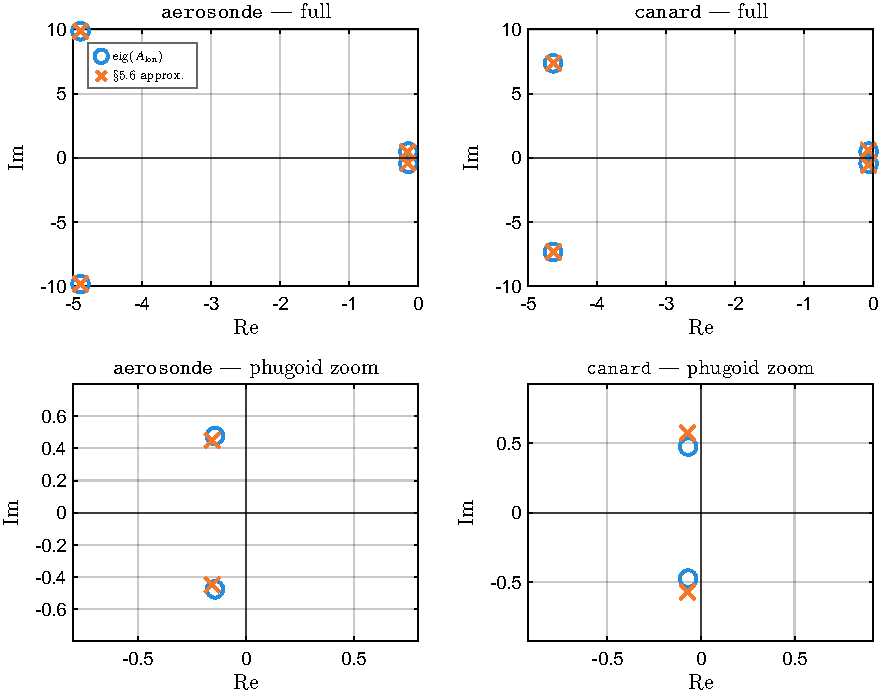
\includegraphics[width=\textwidth]{figs/poles.pdf}
\caption{Longitudinal poles. Circles are eigenvalues of the leading $4\times4$
block of $A_\lon$; crosses are the section 5.6 approximations. The lower row
zooms on the phugoid pair, which is otherwise indistinguishable from the origin
at the scale set by the short-period poles.}
\label{fig:poles}
\end{figure}

\paragraph{Discussion.} The short-period approximation is essentially exact for
both airframes: $11.0059$ against $11.0168\,\mathrm{rad/s}$ for the Aerosonde, an
error of $0.1\%$, and $8.6966$ against $8.7103$ for the canard. This is expected.
The short period is fast enough that airspeed genuinely does not change over one
cycle, so holding $u$ constant is a very good assumption.

The phugoid approximation is markedly worse, and in different directions for the
two airframes: it underestimates the Aerosonde frequency by $4.7\%$ and
overestimates the canard by $20\%$, while getting the damping wrong by $14\%$ and
$12\%$ respectively. This is also expected, and it is the instructive result. The
phugoid is a slow exchange between kinetic and potential energy in which the
angle of attack does vary, so holding $\alpha$ constant discards a real part of
the mechanism. The approximation also neglects $M_u$ and $M_w$ entirely, which the
exact eigenvalues retain.

The practical conclusion is that the short-period approximation is safe to design
against, whereas the phugoid approximation should be treated as an order-of-magnitude
estimate and any phugoid-sensitive design verified against the eigenvalues of
$A_\lon$.

%======================================================================
\section{Longitudinal autopilot}

\subsection{Structure}

Section 6.4 of~\cite{beard} builds the longitudinal autopilot from four loops,
designed inner to outer so that each outer loop sees its inner loop as a
quasi-static gain:

\begin{enumerate}
\item \textbf{Pitch attitude hold on elevator} (\S6.4.1). Proportional-derivative,
  with the rate term taken from the gyro signal $q$ directly rather than by
  differentiating $\theta$:
  $\de = k_{p_\theta}(\theta^c - \theta) - k_{d_\theta}q$.
\item \textbf{Altitude hold on commanded pitch} (\S6.4.2). Proportional-integral,
  outputting $\theta^c$.
\item \textbf{Airspeed hold on commanded pitch} (\S6.4.3). Used in the climb and
  descend regimes.
\item \textbf{Airspeed hold on throttle} (\S6.4.4). Used in the altitude-hold
  regime.
\end{enumerate}

The proportional gain of the inner loop is set so that the elevator just saturates
at the maximum anticipated pitch error, which fixes the pitch bandwidth through
book equation (6.21):
\begin{equation}
  k_{p_\theta} = \frac{\de^{\max}}{e_\theta^{\max}}
                 \operatorname{sign}(a_{\theta_3}),
  \qquad
  \omega_{n_\theta} = \sqrt{a_{\theta_2}
      + \frac{\de^{\max}}{e_\theta^{\max}}\lvert a_{\theta_3}\rvert}.
  \label{eq:kptheta}
\end{equation}
The sign function in~\eqref{eq:kptheta} is required for stability, not cosmetic:
$a_{\theta_3}$ follows $C_{m_{\de}}$, which is negative for both airframes.

Because no integral term is used on the pitch loop, its DC gain is not unity:
\begin{equation}
  K_{\theta_{DC}} = \frac{k_{p_\theta}a_{\theta_3}}
                         {a_{\theta_2} + k_{p_\theta}a_{\theta_3}} ,
  \label{eq:KDC}
\end{equation}
which evaluates to $0.619$ for the Aerosonde. The outer loops must and do account
for this; omitting it is a common source of steady-state altitude error.

The outer loops are separated in bandwidth from the pitch loop by factors $W_h$
and $W_{V_2}$, both set to $10$. A warning is raised if the resulting outer
bandwidths are not in fact below $\omega_{n_\theta}$, since successive loop
closure is invalid otherwise.

\subsection{Altitude state machine}

Following book figure 6.14, the commanded pitch and throttle depend on altitude
error:

\begin{center}
\begin{tabular}{lll}
\toprule
Regime & Throttle & Pitch command \\
\midrule
Take-off & $\dt = 1$ & fixed $\theta^c$ \\
Climb & $\dt = 1$ & from airspeed error \\
Altitude hold & from airspeed error & from altitude error \\
Descend & $\dt = 0$ & from airspeed error \\
\bottomrule
\end{tabular}
\end{center}

Airspeed is regulated with pitch rather than throttle in the climb and descend
regimes, which is what keeps the aircraft away from stall when the throttle is
already saturated. It is deliberately \emph{not} used immediately after take-off,
where pitching down to gain airspeed would fly the aircraft into the ground.

\subsection{Implementation notes}

Two implementation points proved to matter.

Integrator state is carried in an explicit struct passed in and out of the
controller, never in \texttt{persistent} variables. The verification script runs
the control loop more than once per session, and persistent state would make every
run after the first silently wrong.

Each integrator uses conditional integration: the update is accepted only if the
resulting command lies inside its limit, so the integral cannot wind up against a
saturated actuator.

\subsection{Results}

\begin{table}[htbp]
\centering
\begin{tabular}{llrr}
\toprule
Loop & Gain & Aerosonde & Canard \\
\midrule
Pitch (\S6.4.1) & $k_{p_\theta}$ & $-4.5000$ & $-4.5000$ \\
 & $k_{d_\theta}$ & $-0.4877$ & $-0.1904$ \\
 & $K_{\theta_{DC}}$ & $0.6192$ & $0.9464$ \\
 & $\omega_{n_\theta}$ & $16.2004$ & $32.4209$ \\
Altitude (\S6.4.2) & $k_{p_h}$ & $0.1884$ & $0.2467$ \\
 & $k_{i_h}$ & $0.1695$ & $0.4443$ \\
$V_a$ on pitch (\S6.4.3) & $k_{p_{V_2}}$ & $-0.4313$ & $-0.6127$ \\
 & $k_{i_{V_2}}$ & $-0.4321$ & $-1.1317$ \\
$V_a$ on throttle (\S6.4.4) & $k_{p_V}$ & $0.0637$ & $0.0812$ \\
 & $k_{i_V}$ & $0.0264$ & $0.0269$ \\
\bottomrule
\end{tabular}

\caption{Autopilot gains from the section 6.4 formulas, with
$\zeta_\theta = 0.707$, $W_h = W_{V_2} = 10$, $\zeta_h = \zeta_{V_2} = 0.9$,
$\omega_{n_V} = 0.5$.}
\label{tab:gains}
\end{table}

\begin{figure}[htbp]
\centering
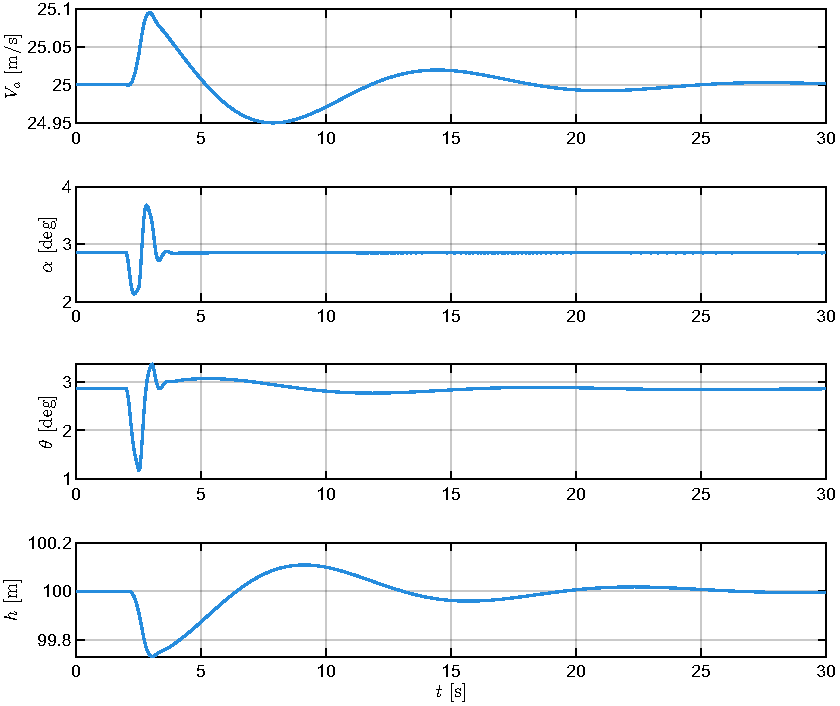
\includegraphics[width=\textwidth]{figs/openloop.pdf}
\caption{Open-loop response of the Aerosonde to a $\pm2^\circ$ elevator doublet
applied at $t=2\,\mathrm{s}$, starting from trim. The fast initial transient is
the short period; the slow lightly damped oscillation in airspeed and altitude
that persists for the rest of the record is the phugoid.}
\label{fig:openloop}
\end{figure}

\begin{figure}[htbp]
\centering
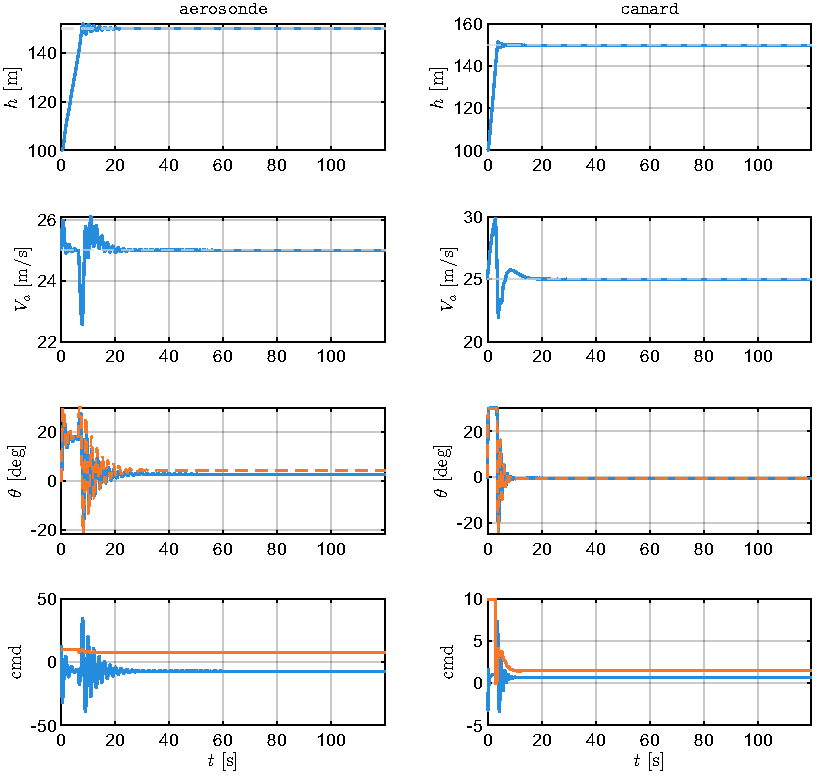
\includegraphics[width=\textwidth]{figs/closedloop.pdf}
\caption{Closed-loop response to a $+50\,\mathrm{m}$ altitude step, both
airframes. Dashed lines are commands. The bottom row shows elevator in degrees
and throttle scaled by ten. Both converge to the commanded altitude with airspeed
returned to its set point.}
\label{fig:closedloop}
\end{figure}

Figure~\ref{fig:openloop} shows the two modes of Section~\ref{sec:modes}
separating cleanly in the time domain, which is an independent confirmation of the
modal analysis. Figure~\ref{fig:closedloop} shows both airframes tracking a
$50\,\mathrm{m}$ altitude step to zero steady-state error while holding airspeed,
with the pitch command visibly saturating during the initial climb and recovering
without integrator windup.

The oscillation visible between roughly $5$ and $25\,\mathrm{s}$ is not a
numerical artefact and is worth naming. It is the altitude state machine
chattering as the aircraft crosses the boundary of the altitude-hold band: within
one band-width of the commanded altitude the controller switches between the climb
law, which commands full throttle and regulates airspeed with pitch, and the hold
law, which regulates altitude with pitch and airspeed with throttle. The two laws
demand different pitch attitudes at the switching point, so repeated crossings
produce the ringing. It decays because each crossing is closer to the command, and
the final tracking error is zero.

This is a known limitation of the switched structure of book figure 6.14 rather
than of the gain design. The standard remedies are hysteresis on the zone
boundaries, or blending the two pitch commands across a transition band instead of
switching discretely. Neither is implemented here, since the chapter 6 structure
was followed as published.

%======================================================================
\section{Verification}\label{sec:verif}

Verification is organised into four groups and automated as a single script that
asserts and throws. All 37 assertions pass. Two of the four groups are
reference-free, which matters because the canard has no published values against
which it could otherwise be checked.

\paragraph{Group 1: trim is a true equilibrium.}
$\lVert f(x^*,u^*)\rVert < 10^{-9}$ for both airframes at $\gamma=0$ and
$\gamma=0.1$; achieved residuals are $\sim\!2\times10^{-15}$. The climb rate is
separately required to satisfy~\eqref{eq:hdotauto}. Including the climbing case is
what gives this group its power: a sign error in the gravity or $\theta$ terms
cancels at $\gamma=0$ and would otherwise go undetected.

\paragraph{Group 2: two independent derivations agree.}
The numerical Jacobian is checked against the closed-form section 5.4
coefficients. $A_\lon(3,3) = -a_{\theta_1}$ and $B_\lon(3,1) = a_{\theta_3}$ hold
exactly for both airframes, and $A_\lon(4,3) = 1$ and $A_\lon(:,5) = 0$ hold to
$10^{-9}$. Agreement between two independent derivations is a stronger statement
than either matching a stored number.

\paragraph{Group 3: against the published reference.}
Table~\ref{tab:verif} summarises. The agreement on $A_\lon$ and $B_\lon$ is the
substantive result: differencing the same way the reference did reproduces its
matrices to within $4\times10^{-5}$ and $1.4\times10^{-10}$ respectively.

\begin{table}[htbp]
\centering
\begin{tabular}{lll}
\toprule
Quantity & Agreement & Evaluated at \\
\midrule
$a_{\theta_1}, a_{\theta_2}, a_{\theta_3}, a_{V_3}$
  & exact to 6--7 significant figures & own trim \\
$a_{V_1}$, $\partial T/\partial V_a$
  & $\sim\!1\times10^{-4}$ relative & reference trim point \\
$a_{V_2}$, $\partial T/\partial\dt$
  & $8.5\times10^{-3}$ relative & reference trim point \\
$A_\lon$ (forward difference, step $0.01$)
  & $3.8\times10^{-5}$ scaled & reference trim point \\
$B_\lon$ (forward difference, step $0.01$)
  & $1.4\times10^{-10}$ scaled & reference trim point \\
\bottomrule
\end{tabular}
\caption{Comparison against published reference values. Quantities that depend on
the trim point are evaluated at the reference's own point, for the reason given in
Section~\ref{sec:refdefects}.}
\label{tab:verif}
\end{table}

The looser agreement on $a_{V_2}$ and $\partial T/\partial\dt$ is attributable to
differencing step rather than to a modelling difference. Thrust is strongly curved
in throttle near cruise, so a coarse forward difference and an accurate central
difference genuinely disagree at the percent level. A hand calculation with a
forward step of $0.01$ gives $90.69$ against the reference $90.279$, while the
converged central-difference value is $89.51$; the reference lies between the two,
consistent with its having been produced by a moderate forward step.

\paragraph{Group 4: closed loop.}
A $10\,\mathrm{m}$ altitude step must settle to within $0.5\,\mathrm{m}$ with
airspeed held to $2\,\mathrm{m/s}$, the pitch command inside its limit and the
throttle inside $[0,1]$, for both airframes. This group is what catches a sign
error in~\eqref{eq:kptheta} or an inverted loop ordering, both of which produce a
model that trims perfectly and then diverges.

One subtlety surfaced here and is worth recording, because the first version of
this check was wrong. The limit $\theta^{\max}$ applies to the pitch
\emph{command}, not to the pitch \emph{state}. A second-order loop with
$\zeta=0.707$ overshoots its command, so $|\theta|$ legitimately exceeds
$\theta^{\max}$ transiently; the canard peaks at $30.09^\circ$ against a
$30^\circ$ limit. The assertion is therefore tight on $\theta^c$ and uses a
$25\%$ band on $\theta$ purely as a divergence guard.

%======================================================================
\section{Defects in the reference material}\label{sec:refdefects}

Three findings about the reference material are recorded here, because each
changed how this work was carried out and the first two would mislead anyone
repeating it.

\subsection{The companion code contains no implemented physics}

The official code companion to~\cite{beard} is a teaching skeleton with every
physics body removed, not a reference implementation. Its trim routine reads, in
full relevant part,
\begin{quote}\ttfamily
state0 = \\
delta0 = \\
x0 = [ state0; delta0 ];
\end{quote}
which is not syntactically valid MATLAB and will not parse. Its state-space
routine is six function headers with six empty bodies; its force-and-moment
function assigns its output from two variables that are never defined. The
repository README confirms that worked solutions are distributed to instructors
only.

Consequently nothing in this work is ported from it. All equations are taken from
the text. The companion material contributed exactly two usable things: the
Aerosonde parameter values, and a file of published numerical results used here as
a verification oracle.

\subsection{The published trim point is not a force equilibrium}

Evaluating the dynamics at the published $x^*$ and $u^*$ gives
$\dot u = -0.85\,\mathrm{m/s^2}$, not zero. The cause is traceable: at
$\dt = 0.6768$ and $V_a = 25\,\mathrm{m/s}$ the propeller model
of~\eqref{eq:propquad} delivers about $0.95\,\mathrm{N}$ of thrust, whereas the
drag at that condition is $10.3\,\mathrm{N}$. The equilibrium throttle is
$0.7734$, which is what the trim routine here returns. This is consistent with the
companion repository's own README, which notes parameter difficulties and
recommends $V_a = 35\,\mathrm{m/s}$ for this airframe.

The published $A_\lon$ and $B_\lon$ remain internally consistent, because a
Jacobian and the analytic coefficients are both defined at a point and neither
requires that point to be an equilibrium. This is precisely why
$a_{\theta_1}$ through $a_{\theta_3}$ matched immediately while $a_{V_1}$ and
$a_{V_2}$ did not: the former depend only on $V_a$ and the airframe, the latter on
the trim point.

The verification strategy follows from this. Trim is not compared against the
published point at all. Instead the Jacobian is evaluated \emph{at} the published
point for an exact comparison of $A_\lon$ and $B_\lon$, while the trim routine is
separately required to produce a genuine equilibrium. Both checks are then tight,
rather than one being confounded by the other.

\subsection{The shipped parameter sets disagree with each other}

The companion repository ships two copies of the same aircraft whose drag
parameters differ materially:

\begin{center}
\begin{tabular}{lrr}
\toprule
 & MATLAB copy & Python copy \\
\midrule
$C_{D_0}$ & $0.043$ & $0.0424$ \\
$C_{D_\alpha}$ & $0.030$ & $\mathbf{0.132}$ \\
$C_{D_p}$ & $0.0$ & $0.043$ \\
$c$ & $0.19$ & $0.18994$ \\
\bottomrule
\end{tabular}
\end{center}

$C_{D_\alpha}$ differs by a factor of $4.4$, which is not a rounding difference.
The published reference values were generated with the Python set. This was
settled by direct computation rather than by inspection: substituting into
\eqref{eq:aV},
\begin{equation}
  a_{V_1} = \frac{1.2682 \times 25 \times 0.55}{11}
            \bigl(0.0424 + 0.132(0.05001) + 0.0135(-0.12478)\bigr)
            + \frac{2.3522}{11} = 0.288845,
  \label{eq:aV1check}
\end{equation}
against the published $0.2888454$, agreeing to seven significant figures. The
MATLAB values do not reproduce it. The parameter file used here therefore carries
the Python numbers, with an explicit warning comment against ``correcting'' them
back.

Equation~\eqref{eq:aV1check} also settles two secondary questions at once. It
confirms the linear-in-$\alpha$ drag law of~\eqref{eq:dragpoly} rather than the
induced-drag polar, and the magnitude of its propulsive term confirms the
addendum propeller model rather than the legacy one.

%======================================================================
\section{Conclusions}

The longitudinal design chain of~\cite{beard} chapters 3 to 6 has been
implemented in full and verified. The principal results are:

\begin{itemize}
\item Trim is solved to a residual of $\sim\!2\times10^{-15}$ for both airframes,
  at level and climbing conditions, using two scalar root-finds rather than a
  constrained optimiser. Exploiting the triangular structure of the problem
  removes the Optimization Toolbox dependency and improves the residual by nine
  orders of magnitude over a tolerance-based solve.
\item The linearised model reproduces published reference matrices to
  $3.8\times10^{-5}$ and $1.4\times10^{-10}$, and the analytic transfer function
  coefficients to seven significant figures.
\item The short-period approximation of section 5.6 is accurate to $0.1\%$ and
  safe to design against. The phugoid approximation errs by $5$ to $20\%$ in
  frequency and should be treated as indicative only.
\item The successive-loop-closure autopilot tracks altitude steps to zero
  steady-state error on both airframes while holding airspeed, with the
  inner-loop DC gain of~\eqref{eq:KDC} correctly propagated to the outer loops.
\end{itemize}

Two defects in the reference material were identified and documented: a companion
codebase with no implemented physics, and a published trim point that is not a
force equilibrium. The second of these required restructuring the verification so
that reference comparison and equilibrium verification are separate, independently
tight checks rather than a single confounded one.

The natural extensions are the lateral chain, which would reuse the trim and
linearisation machinery essentially unchanged, and atmospheric disturbance, which
enters as an additive term on $V_a$ and $\alpha$ and would leave the rest of the
structure intact.

%======================================================================
\appendix
\section{Software}

Eleven MATLAB files, roughly 1300 lines, with no toolbox dependencies.

\begin{center}
\begin{tabular}{lll}
\toprule
File & Chapter & Purpose \\
\midrule
\texttt{lon\_params.m} & --- & Both airframes, one canonical struct \\
\texttt{f\_lon.m} & 3, 4 & Nonlinear EOM, forces, both thrust models \\
\texttt{compute\_lon\_trim.m} & 5.3, F.2 & Trim \\
\texttt{compute\_lon\_ss.m} & 5.5, F.4 & Finite-difference Jacobian \\
\texttt{compute\_lon\_tf.m} & 5.4 & Transfer functions and coefficients \\
\texttt{lon\_modes.m} & 5.6 & Modal analysis, exact and approximate \\
\texttt{lon\_gains.m} & 6.4 & Gain design \\
\texttt{lon\_autopilot.m} & 6.4 & Four loops and the state machine \\
\texttt{lon\_autopilot\_reset.m} & 6.4 & Integrator state \\
\texttt{run\_lon.m} & --- & Driver \\
\texttt{check\_lon.m} & --- & 37 verification assertions \\
\bottomrule
\end{tabular}
\end{center}

Reproduce the results of this report with
\begin{quote}\ttfamily
run\_lon \\
check\_lon
\end{quote}
and regenerate its tables and figures with \texttt{make\_report\_data} from the
report directory.

\begin{thebibliography}{9}
\bibitem{beard}
R.~W.~Beard and T.~W.~McLain,
\emph{Small Unmanned Aircraft: Theory and Practice},
Princeton University Press, 2012.
\end{thebibliography}

\end{document}
